\documentclass[tikz,border=8pt]{standalone}
\usetikzlibrary{automata,positioning,arrows.meta,fit,backgrounds}
\begin{document}
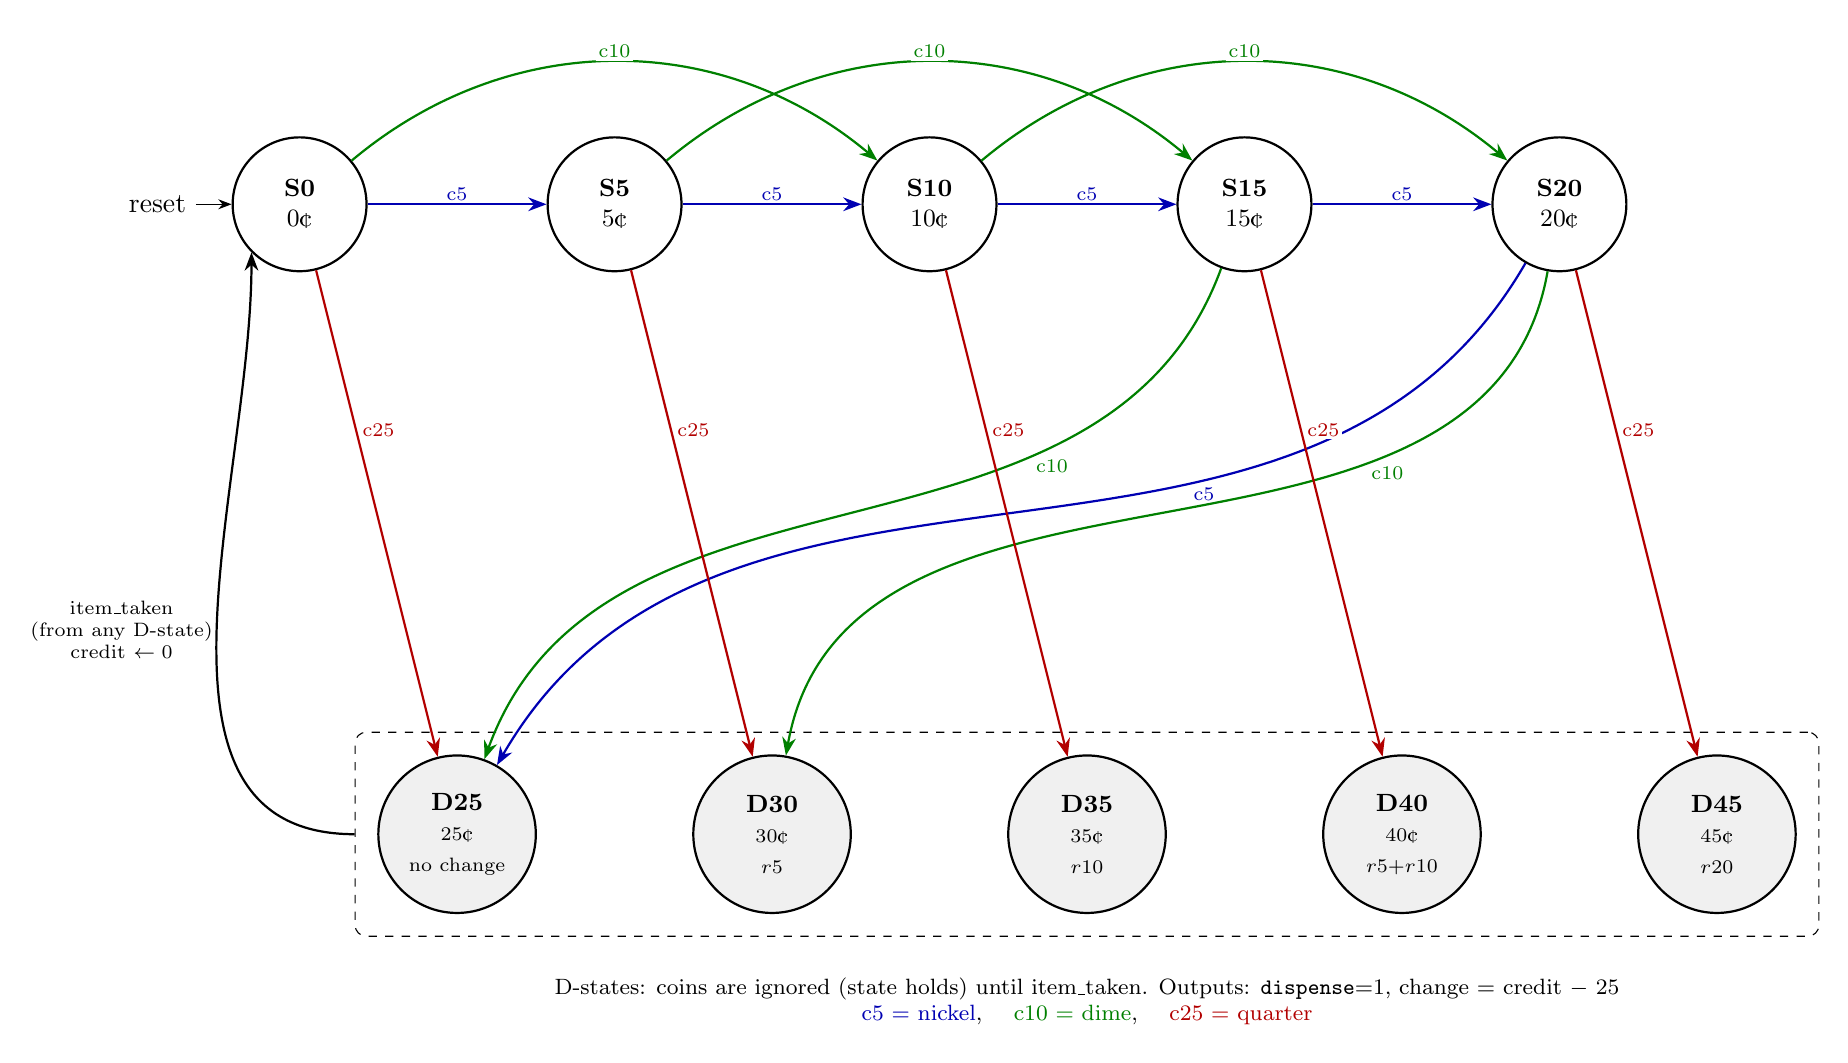
\begin{tikzpicture}[>=Stealth, auto,
  st/.style={circle, draw, thick, minimum size=1.7cm, align=center, font=\small, inner sep=1pt},
  dst/.style={circle, draw, thick, minimum size=2.0cm, align=center, font=\small, inner sep=1pt, fill=gray!12},
  c5/.style={->, thick, blue!70!black},
  c10/.style={->, thick, green!50!black},
  c25/.style={->, thick, red!70!black},
  lbl/.style={font=\scriptsize, fill=white, inner sep=1pt, pos=0.5}]

  % COLLECT states (credit = 0..20)
  \node[st, initial, initial text=reset] (S0)  at (0,0)  {\textbf{S0}\\ $0$\textcent};
  \node[st] (S5)  at (4,0)  {\textbf{S5}\\ $5$\textcent};
  \node[st] (S10) at (8,0)  {\textbf{S10}\\ $10$\textcent};
  \node[st] (S15) at (12,0) {\textbf{S15}\\ $15$\textcent};
  \node[st] (S20) at (16,0) {\textbf{S20}\\ $20$\textcent};

  % DISPENSE states (credit = 25..45)
  \node[dst] (D25) at (2,-8)  {\textbf{D25}\\ \scriptsize $25$\textcent\\ \scriptsize no change};
  \node[dst] (D30) at (6,-8)  {\textbf{D30}\\ \scriptsize $30$\textcent\\ \scriptsize $r5$};
  \node[dst] (D35) at (10,-8) {\textbf{D35}\\ \scriptsize $35$\textcent\\ \scriptsize $r10$};
  \node[dst] (D40) at (14,-8) {\textbf{D40}\\ \scriptsize $40$\textcent\\ \scriptsize $r5{+}r10$};
  \node[dst] (D45) at (18,-8) {\textbf{D45}\\ \scriptsize $45$\textcent\\ \scriptsize $r20$};

  % nickel (c5)
  \draw[c5] (S0)  -- node[lbl]{c5}  (S5);
  \draw[c5] (S5)  -- node[lbl]{c5}  (S10);
  \draw[c5] (S10) -- node[lbl]{c5}  (S15);
  \draw[c5] (S15) -- node[lbl]{c5}  (S20);
  \draw[c5] (S20) to[out=-120,in=60] node[lbl,pos=0.35]{c5} (D25);

  % dime (c10)
  \draw[c10] (S0)  to[bend left=40] node[lbl]{c10} (S10);
  \draw[c10] (S5)  to[bend left=40] node[lbl]{c10} (S15);
  \draw[c10] (S10) to[bend left=40] node[lbl]{c10} (S20);
  \draw[c10] (S15) to[out=-110,in=70] node[lbl,pos=0.3]{c10} (D25);
  \draw[c10] (S20) to[out=-100,in=80] node[lbl,pos=0.3]{c10} (D30);

  % quarter (c25)
  \draw[c25] (S0)  -- node[lbl,pos=0.35]{c25} (D25);
  \draw[c25] (S5)  -- node[lbl,pos=0.35]{c25} (D30);
  \draw[c25] (S10) -- node[lbl,pos=0.35]{c25} (D35);
  \draw[c25] (S15) -- node[lbl,pos=0.35]{c25} (D40);
  \draw[c25] (S20) -- node[lbl,pos=0.35]{c25} (D45);

  % return to S0
  \begin{scope}[on background layer]
    \node[draw, dashed, rounded corners, fit=(D25)(D30)(D35)(D40)(D45), inner sep=8pt] (box) {};
  \end{scope}
  \draw[->, thick] (box.west) to[out=180,in=-90] node[lbl,pos=0.5,align=center]{item\_taken\\ (from any D-state)\\ credit $\leftarrow 0$} (S0.south west);

  \node[font=\footnotesize, align=center, below=0.4cm of box] {
    D-states: coins are ignored (state holds) until item\_taken. Outputs: \texttt{dispense}=1,
    change = credit $-$ 25 \\
    {\color{blue!70!black}c5 = nickel}, \quad {\color{green!50!black}c10 = dime}, \quad {\color{red!70!black}c25 = quarter}};
\end{tikzpicture}
\end{document}
